\subsection*{Solution to Fall 2013, \#1}
\label{F13Q1}

\subsubsection*{Solution to $1a$ and $1b$}

Since $\psi(x) = \frac{1}{2} (x^2-1)^2$, the ODE system is
$$ \left\{
\begin{array}{l}
x_t = v \\
v_t = -2x(x^2-1) - \alpha v
\end{array}
\right.
$$
Hence, the stationary points are $(-1,0)$, $(0,0)$, and $(1,0)$. Furthermore the Jacobian of the system is
$$ J(x,y) = \pmat{0}{1}{-6x^2 + 2}{-\alpha} $$
Then, we compute the eigenvalues and eigenvectors. For $J(0,0)$, the eigenvalues are $\frac{-\alpha \pm \sqrt{\alpha^2 + 8}}{2}$. For $J(\pm 1,0)$, we have that
the eigenvalues are $\frac{-\alpha \pm \sqrt{\alpha^2 - 16}}{2}$.
From the eigenvalues, $(0,0)$ will always be a saddle, while $(\pm 1, 0)$ depends on the value of $\alpha$.

If $0 < \alpha < 4$, then $(\pm 1, 0)$ are inward pointing spirals. Below is a phase plane plot for $\alpha = 1$.
\begin{center}
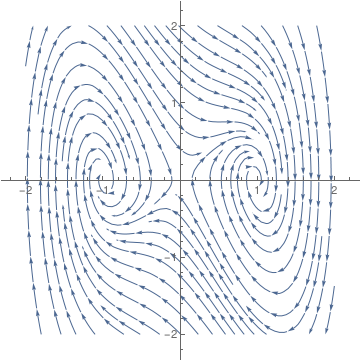
\includegraphics[scale=0.75]{./_Figures/f1311.png}
\end{center}

If $\alpha = 4$, then $(\pm 1, 0)$ are nodes (the eigenvalues for $J(\pm 1, 0)$ are repeated). Below is a phase plane plot for $\alpha = 4$.
\begin{center}
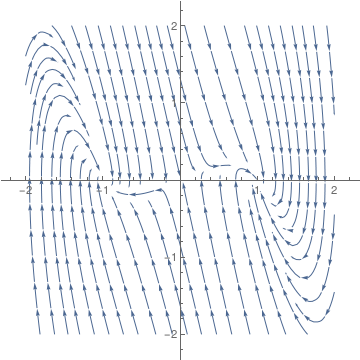
\includegraphics[scale=0.75]{./_Figures/f1312.png}
\end{center}

If $\alpha > 4$, then $(\pm 1, 0)$ are sinks. Below is a phase plane plot for $\alpha = 6$.
\begin{center}
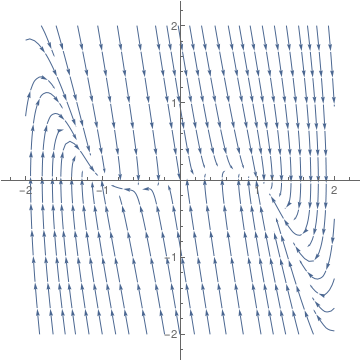
\includegraphics[scale=0.75]{./_Figures/f1313.png}
\end{center}

\subsubsection*{Solution to $1c$}

To how $H$ is non-increasing with time, we take a time derivative. Same as in parts (a) and (b), we assume $\alpha < 0$.
$$ \dot{H}(x,v) = v \dot{v} + \psi'(x) \dot{x} = v(-2x(x^2-1)-\alpha v) + 2xv(x^2-1) = -\alpha v^2 < 0 $$
Hence, $H$ is non-increasing with time. \hfill \qed


\subsection*{Solution to Fall 2013, \#2}
\label{F13Q2}

\subsubsection*{Solution to $2a$}
	
First, observe that, with the given choice of $f$, $E$ can be succinctly written as
\begin{equation}
	\label{F13Q2one}
	E(u) = \frac{1}{2} \int_{\Omega} \abs{\del u}^2 + gu \,dx + \frac{1}{2} \int_{\d \Omega} u^2 \, dS(x)
\end{equation}
Now, suppose $u$ minimizes \eqref{F13Q2one}, and let $v \in H^1(\Omega)$. We compute
$$ \frac{1}{\epsilon} \left(E(u+\epsilon v) - E(u) \right) = \int_{\Omega} \del u \cdot \del v + \epsilon v^2 + gv \,dx + \int_{\d \Omega} u v + \epsilon v^2 \, dS(x) $$
Since $u$ is a minimizer of $E$, sending $\epsilon \to 0$ yields
$$ \int_{\Omega} \del u \cdot \del v + gv \,dx + \int_{\d \Omega} u v \, dS(x) = 0 \quad \Leftrightarrow \quad \int_{\Omega} \del u \cdot \del v \, dx + \int_{\d \Omega} u v \, dS(x) = - \int_{\Omega} gv \, dx $$
Define the bilinear form $B : H^1(\Omega) \times H^1(\Omega) \to \R$ as
$$ B[u,v] = \int_{\Omega} \del u \cdot \del v \, dx + \int_{\d \Omega} uv \, dS(x) $$
and the function $F : H^1(\Omega) \to \R$ as
$$ F(v) = -\int_{\Omega} gv \, dx $$
Assuming $g \in L^2(\Omega)$, it's straightforward to check that both $B$ and $F$ are bounded:
\begin{align*}
	|B[u,v]| &\leq \nm{\del u}_{L^2(\Omega)} \nm{\del v}_{L^2(\Omega)} + \nm{u}_{L^2(\d \Omega)} \nm{v}_{L^2(\d \Omega)} \\
	&\leq 2 \nm{u}_{H^1(\Omega)} \nm{v}_{H^1(\Omega)}
\end{align*}
and
$$ |F(v)| \leq \nm{g}_{L^2(\Omega)} \nm{v}_{L^2(\Omega)} \leq C \nm{v}_{H^1(\Omega)} $$
(Note: In order to show $B$ is bounded, we invoked the Trace Theorem, which states $\nm{u}_{L^2(\d \Omega)} \leq \nm{u}_{H^1(\Omega)}$.) Furthermore, $B$ is symmetric and satisfies the property $B[u,u] \geq 0$ for all $u \in H^1(\Omega)$ and $B[u,u] = 0$ if $u \equiv 0$. If $B[u,u] = 0$, then $\del u \equiv 0$ in $\Omega$ and $u \equiv 0$ on $\d \Omega$. The condition on the derivative implies $u$ must be constant, and pairing this with the condition on the boundary implies $u \equiv 0$. Thus, $B$ defines an inner product on $H^1(\Omega)$, and by the Riesz Representation Theorem, there exists a unique $u \in H^1(\Omega)$ such that
\begin{equation}
\label{F13Q2two}
	B[u,v] = F(v) \quad \forall v \in H^1(\Omega)
\end{equation}

Now, we reverse the work we've done to obtain the result. Define $B$ and $F$ as stated above, and observe that there exists a unique $u \in H^1(\Omega)$ such that \eqref{F13Q2two} holds. Because of how we defined $B$ and $F$, $u$ must be the unique critical point of $E$. Finally, since $E$ is convex, $u$ must minimize $E$. Therefore, $E$ has a unique minimizer in $H^1(\Omega)$.  \hfill \qed

\subsubsection*{Solution to $2b$}

Recall from our work above that the minimizer $u$ of $E$ must satisfy
$$ \int_{\Omega} \del u \cdot \del v + gv \,dx + \int_{\d \Omega} u v \, dS(x) = 0 $$
for all $v \in H^1(\Omega)$. Applying integration by parts to the first term above yields
$$ \int_{\Omega} -\Delta u v \, dx + \int_{\d \Omega} \frac{\d u}{\d \nu} v \, dS(x) + \int_{\Omega} gv \, dx + \int_{\d \Omega} uv \, dS(x) = 0 $$
Since this holds for all $v \in H^1(\Omega)$, we obtain the following differential equation and boundary condition for the minimizer of $E$:
$$ \Delta u = g \quad \text{in} \,\, \Omega $$
$$ \frac{\d u}{\d \nu} + u = 0 \quad \text{on} \,\, \d \Omega $$
\hfill \qed

\subsubsection*{Solution to Fall 2013, \#2$(a)$ with Lax-Milgram}
Let
\begin{align*}
B[u, v] := \int_{\Om}\nabla u \cdot \nabla v\, dx + \int_{\pr \Om}uv\, d\sigma \quad \text{ and } \quad \psi(v) := \int_{\Om} -g v\, dx.
\end{align*}
Note
$$|B[u, v]| \leq \nms{\nabla u}_{L^{2}(\Om)}\nms{\nabla v}_{L^{2}(\Om)} + \|u\|_{L^{2}(\pr \Om)}\|v\|_{L^{2}(\pr \Om)} \leq C\|u\|_{H^{1}(\Om)}\|v\|_{H^{1}(\Om)}$$
by the boundedness of the trace operator (strictly speaking, we should really be writing $\|Tu\|_{L^{2}(\pr \Om)}$ instead of $\|u\|_{L^{2}(\pr \Om)}$ where
$T: H^{1}(\Om) \rightarrow L^{2}(\pr \Om)$ where $T$ is the trace operator). As $g \in L^{2}$,
$$|\psi(v)| \leq \|g\|_{L^{2}(\Om)}\|v\|_{L^{2}(\Om)} \leq \|g\|_{L^{2}(\Om)}\|v\|_{H^{1}(\Om)}$$
and so $\psi$ is a bounded linear functional on $H^{1}(\Om)$.

To prove existence of a weak solution, it now remains to show that $B[u, v]$ is coercive (that is, there exists a $\beta$ such that
$\beta \|u\|_{H^{1}}^{2} \leq B[u, u]$ for all $u \in H^{1}$). Suppose $B$ was not coercive, then there exists
$\{u_{n}\}$ such that $\nms{u_{n}}_{H^{1}(\Om)} = 1$ and $B[u_{n}, u_{n}] \rightarrow 0$ as $n \rightarrow \infty$.
By weak compactness, there exists a subsequence $\{u_{n_{k}}\} \subset \{u_{n}\}$ and a $u \in H^{1}(\Om)$ such that
$u_{n_{k}} \rightharpoonup u$ as $k \rightarrow \infty$ in $H^{1}(\Om)$. Since a weakly convergent sequence is bounded and by
Rellich-Kondrachov, $H^{1}(\Om)$ embeds compactly into $L^{2}(\Om)$, we have a further subsequence such that
$u_{n_{k_{j}}} \rightarrow u$ as $n_{k_{j}} \rightarrow \infty$ in $L^{2}(\Om)$.

We have
\begin{align}\label{altf132eq1}
B[u_{n_{k_{j}}}, u_{n_{k_{j}}}] = \int_{\Om}|\nabla u_{n_{k_{j}}}|^{2}\, dx + \int_{\pr \Om}u_{n_{k_{j}}}^{2}\, d\sigma \rightarrow 0.
\end{align}
Thus
$$\int_{\Om}|\nabla u_{n_{k_{j}}}|^{2}\, dx \rightarrow 0$$
as $n_{k_{j}} \rightarrow \infty$.
Since $u_{n_{k}} \rightharpoonup u$ in $H^{1}(\Om)$,
\begin{align}\label{altf132}
\int_{\Om}(u_{n_{k_{j}}} - u)v\, dx + \int_{\Om}\nabla(u_{n_{k_{j}}} - u)\cdot \nabla v\, dx \rightarrow 0
\end{align}
for all $v \in H^{1}(\Om)$. Indeed, for each $v \in H^{1}(\Om)$, let $L_{v} : H^{1}(\Om) \rightarrow \R$ be defined by
$$L_{v}(u) := \int_{\Om}uv\, dx + \int_{\Om}\nabla u \cdot \nabla v\, dx.$$ Since $u_{n_{k}}\rightharpoonup u$, $L_{v}(u_{n_{k}}) \rightarrow L_{v}(u)$ which
proves \eqref{altf132}.
Then as $u_{n_{k_{j}}} \rightarrow u$ in $L^{2}(\Om)$, taking $v = u$ in \eqref{altf132} yields
$$\int_{\Om}|\nabla u|^{2}\, dx = \lim_{n_{k_{j}} \rightarrow \infty}\int_{\Om}\nabla u_{n_{k_{j}}} \cdot \nabla u = 0.$$
Therefore $\nms{u}_{H^{1}(\Om)} = \nms{u}_{L^{2}(\Om)}$. Then
$$\nms{u}_{L^{2}(\Om)} = \lim_{n_{k_{j}} \rightarrow \infty}\nms{u_{n_{k_{j}}}}_{L^{2}(\Om)} = 1.$$
Since $\int_{\Om}|\nabla u|^{2}\, dx = 0$, $u$ is constant on $\Om$. Since $\|u\|_{L^{2}(\Om)} = 1$, $u = c \neq 0$.

However, by \eqref{altf132eq1}
$$\int_{\pr \Om}u^{2}\, d\sigma = \lim_{n_{k_{j}} \rightarrow \infty}\int_{\pr \Om}u_{n_{k_{j}}}^{2}\, d\sigma = 0,$$
(here we are once again abusing notation and we should be writing $Tu$ and $Tu_{n_{k_{j}}}$ instead, the above equation is essentially
the fact that trace is a continuous linear operator) and hence $u = 0$ on $\pr \Om$, a contradiction since $u = c \neq 0$ in $\Om$.
Thus $B$ is coercive. Thus by Lax-Milgram, there exists a unique $\wt{u} \in H^{1}(\Om)$ such that $B[\wt{u}, v] = \psi(v)$ for all $v \in H^{1}(\Om)$.
\hfill\qed

\subsection*{Solution to Fall 2013, \#3}
\label{F13Q3}

We solve this using method of characteristics. Because the PDE is quasilinear, we only need to solve the following ODEs to obtain our solution:
\begin{align}
\label{F13Q3Eqt} &\dot t(s) = 1, \quad t(0) = 0 \\
\label{F13Q3Eqx} &\dot x(s) = f'(z(s)), \quad x(0) = x_0 \\
\label{F13Q3Eqz} &\dot z(s) = 0, \quad z(0) = \phi(x_0) = -x_0 \\
\end{align}
Solving \eqref{F13Q3Eqt} and \eqref{F13Q3Eqz} yield
$$ t(s) = s, \quad z(s) = -x_0 $$
respectively. Then, solving \eqref{F13Q3Eqx} yields
$$ x(s) = f'(-x_0)t + x_0 $$
This implies
$$ u(x,t) = -x_0, \quad \text{where} \,\,\, x = f'(-x_0)t + x_0 $$
Taking a partial derivative of $u$ with respect to $x$ yields $u_x = -\frac{\d x_0}{\d x}$. Next, we compute
\begin{align*}
\frac{\d}{\d x} \left[ x = f'(-x_0)t + x_0 \right] \quad &\implies \quad 1 = -f''(-x_0)t \frac{\d x_0}{\d x} + \frac{\d x_0}{\d x} \\
&\implies \quad \frac{\d x_0}{\d x} = \frac{1}{1 - f''(-x_0)t}
\end{align*}
Thus,
$$ |u_x(x,t)| = \frac{1}{|1-f''(-x_0)t|} $$
Since $f''(u) \geq \theta > 0$ for all $u$, we know that, by the time $t = 1/\theta$, the expression $1-f''(-x_0)t$ will have already equaled 0. Therefore, $|u_x| \to \infty$ in finite time. \hfill \qed



\subsection*{Solution to Fall 2013, \#4}
\label{F13Q4}

We think there is a typographical error in the problem statement. Specifically, we think the PDE should read
$$ u_{tt} + c^2 u_{xxxx} + au_t = 0 $$
(a plus sign instead of a minus sign between the first two terms). Our solution reflects this change.

\subsubsection*{Solution to $4a$}

If this is indeed the intended PDE, define the energy
$$ E(t) := \frac{1}{2} \int_{\R} u_t^2 + c^2 u_{xx}^2 \, dx $$
Then,
$$ \dot{E}(t) = \int_{\R} u_t u_{tt} + c^2 u_{xx} u_{xxt} \, dx $$
Since we're assuming solutions have compact support, two application of integration by parts yields
$$ \dot{E}(t) = \int_{\R} u_t u_{tt} + c^2 u_{xxxx}u_t \, dx = \int_{\R} -a u_t^2 \, dx \leq 0 $$
Hence, the energy is non-increasing with time. \hfill \qed

\subsubsection*{Solution to $4b$}

Let $u$ and $v$ be solutions with compactly supported initial data, and consider $ w:= u-v$. Observe that $w$ satisfies
$$ \left\{
\begin{array}{lll}
w_{tt} + c^2 w_{xxxx} + aw_t = 0 \\
w(x,0) = 0 \\
w_t(x,0) = 0
\end{array}
\right. $$
Furthermore, since both $u$ and $v$ are compactly supported, $w$ is as well (see remark below). Thus, defining the energy as
$$ E(t) := \frac{1}{2} \int_{\R} w_t^2 + c^2 w_{xx}^2 \, dx $$
and using the same argument as in $4a$ yields $\dot{E}(t) \leq 0$. Furthermore, observe that $E(0) = 0$. Finally, because $E(t) \geq 0$ for all time, we must have that $E(t) \equiv 0$ for all time. This implies $w_t \equiv 0$ and $w_{xx} \equiv 0$. This implies that $w(x,t) = f(x)$, a function dependent only on $x$. Since $w_{xx} \equiv 0$, we know $f''(x) = 0$, implying that $w(x,t) = ax+b$ for some $a, b \in \R$. Then, $w(x,0) = 0$ implies $b=0$. Now, $0 = w(x,0) = ax$ implies $a = 0$, too. We've shown $w \equiv 0$, and therefore, solutions are unique. \hfill \qed

\begin{rem}
In the solution, we stated without proof that solutions with compactly supported initial data must be compactly supported. This can be shown by following Evans' proof of the domain of dependence for the wave equation (pg. 84, 2nd edition), but with the use of the energy defined for this problem.
\end{rem}


\subsection*{Solution to Fall 2013, \#5}
\label{F13Q5}

First, let's assume $4aT < 1$. Then, there exists $\delta > 0$ and $\gamma > 0$ such that
$$ 4a(T+\delta) < 1 \quad \text{and} \quad \frac{1}{4(T+\delta)} = a + \gamma $$
Fix an arbitrary $y \in \R$ and $\epsilon > 0$. Let
$$ v(x,t) := u(x,t) - \frac{\epsilon}{(T+\delta -t)^{1/2}} e^{\frac{(x-y)^2}{4(T+\delta - t)}} $$
Then, observe that
\begin{align*}
\frac{\d}{\d t} (T-\delta - t)^{-1/2} e^{\frac{(x-y)^2}{4(T+\delta - t)}} &= \left[ \frac{1}{2} \frac{1}{(T+\delta -t)^{3/2}} + \frac{1}{4} \frac{(x-y)^2}{(T+\delta - t)^{5/2}}\right]  e^{\frac{(x-y)^2}{4(T+\delta - t)}} \\
&= \frac{\d^2}{\d x^2} (T-\delta - t)^{-1/2} e^{\frac{(x-y)^2}{4(T+\delta - t)}}
\end{align*}
so we have $v_t - v_{xx} = 0$ in $\R \times (0,T]$. Let $r > 0$ be sufficiently large to be chosen later and let $U := B_r(y)$, $U_T := B_r(y) \times (0,T]$. Then, by the maximum principle for the heat equation
\begin{equation}
\label{f135max}
\max_{\overline{U_T}} v = \max_{\Gamma_T} v
\end{equation}
where $\Gamma_T := \overline{U_T} \bs U_T$.
Note that
$$ v(x,0) = u(x,0) - \frac{\epsilon}{(T+\delta)^{1/2}} e^{\frac{(x-y)^2}{4(T+\delta)}} \leq u(x,0) = 0 $$
and for $x$ such that $|x-y| = r$, we have
\begin{align*}
v(x,t) &= u(x,t) - \frac{\epsilon}{(T+\delta -t)^{1/2}} e^{\frac{(x-y)^2}{4(T+\delta - t)}} \\
&\leq Ce^{ax^2} - \frac{\epsilon}{(T+\delta -t)^{1/2}} e^{\frac{r^2}{4(T+\delta - t)}} \\
&\leq Ce^{ax^2} - \frac{\epsilon}{(T+\delta)^{1/2}} e^{\frac{(x-y)^2}{4(T+\delta)}} \\
&\leq Ce^{a(|y|+r)^2} - \epsilon (4(a+\gamma))^{1/2} e^{(a+\gamma)r^2} \leq 0
\end{align*}
if $r$ is sufficiently large. Thus, by \eqref{f135max} and the arbitrariness of $y$, $v(y,t) \leq 0$ for all $0 \leq t \leq T$ and $y \in \R^n$. Letting $\epsilon \to 0$ shows that $u(x,t) \leq 0$ for all $x \in \R^n$, $0 \leq t \leq T$. Replacing $u$ with $-u$ shows that $u(x,t) = 0$ for all $x \in \R^n$, $0 \leq t \leq T$ if $4aT < 1$.

If $4aT \geq 1$, then we repeatedly apply the result on the time intervals $[0,T_1], [T_1,2T_1], \dots$ for $T_1 = \frac{1}{8a}$. \hfill \qed



\subsection*{Solution to Fall 2013, \#6}
\label{F13Q6}

Suppose $u$ is a solution of the given PDE. As the equation looks like a nonlinear version
of the transport equation, let $z(s) := u(x - s, t + s)$. Then
$$\dot{z}(s) = u_{x}(x - s, t + s)(-1) + u_{t}(x - s, t + s) = -u^{2}(x - s, t + s)$$
and hence
$$u(x, t) - \psi(x + t) = z(0) - z(-t) = \int_{-t}^{0}-u^{2}(x - s, t + s)\, ds = \int_{0}^{t}-u^{2}(x - s + t, s)\, ds.$$
Then
$$u(x, t) = \psi(x + t) - \int_{0}^{t}u^{2}(x - s + t, s)\, ds.$$
Therefore a solution to the given PDE is a fixed point of the operator
$$F(\vp)(x, t) := \psi(x + t) - \int_{0}^{t}\vp^{2}(x - s + t, s)\, ds$$
where $\vp \in \textrm{BC}(\R^{2} \rightarrow \R)$, the bounded continuous functions from $\R^{2} \rightarrow \R$
which is a complete metric space under the sup norm $\nms{\cdot}_{\infty}$.
Since $\psi$ is smooth with compact support, $\nms{\psi}_{\infty} = \sup_{x \in \R}\abn{\psi(x)} < \infty$.
Let $T$ be such that $T\nms{\psi}_{\infty} \leq 1/100$. Then
\begin{align}
\label{F13Q6one}
\nms{F(\vp)}_{\infty} \leq \nms{\psi}_{\infty} + T\nms{\vp}_{\infty}^{2} \leq \nms{\psi}_{\infty} + \frac{1}{100\nms{\psi}_{\infty}}\nms{\vp}_{\infty}^{2}.
\end{align}

Let $V := \{\vp \in \textrm{BC}(\R^{2} \rightarrow \R): \|\vp\|_{\infty} \leq 2\|\psi\|_{\infty}\}$.
Since $V$ is a closed subset of $\textrm{BC}(\R^{2} \rightarrow \R)$, $V$ is complete.
We will show that
$F: V \rightarrow V$ and that $F$ is a contraction on $V$. Explicitly, we will show that $F(\vp) \in V$ for all $\vp \in V$
and for any $\vp, \phi \in V$, $\|F(\vp) - F(\phi)\|_{\infty} \leq \alpha \|\vp - \phi\|_{\infty}$ for some $\alpha < 1$.

We first show that $F(\vp) \in V$ for all $\vp \in V$. By \eqref{F13Q6one}, we have
\begin{align*}
\|F(\vp)\|_{\infty} \leq \|\psi\|_{\infty} + \frac{1}{100\nms{\psi}_{\infty}}4\|\psi\|_{\infty}^{2} < 2\|\psi\|_{\infty}
\end{align*}
and hence $F(\vp) \in V$. Next,
\begin{align*}
\|F(\vp) - F(\phi)\|_{\infty} &= \bigg\|\int_{0}^{t}\phi(x - s + t, s)^{2} - \vp(x - s + t, s)^{2}\, ds\bigg\|_{\infty}\\
&\leq 4T\|\psi\|_{\infty}\|\phi - \vp\|_{\infty} \leq \frac{1}{25}\|\phi - \vp\|_{\infty}.
\end{align*}

Thus $F$ is a contraction on $V$. Therefore there exists a unique fixed point in $V$. Since fixed points of
$F$ are solutions to the PDE, there exists a unique solution to the PDE if $T$ is chosen sufficiently small. \hfill\qed

\subsection*{Solution to Fall 2013, \#7}
\label{F13Q7}

Based on the information given in the problem, we don't know whether or not $u$ is continuous at the origin. If it is, we will show that $u$ is harmonic in all of $\R^3$, and if not, we will show that $u$ can be harmonically extended to all of $\R^3$.

Let $v$ satisfy the following conditions
$$ \left\{
\begin{array}{ll}
\Delta v = 0 & \text{in} \,\, B_1(0) \\
v = u & \text{on} \,\, \d B_1(0)
\end{array} \right. $$
where $u$ is the function defined in the problem statement. Let $w := u-v$, and observe that $w$ satisfies
$$ \left\{
\begin{array}{ll}
\Delta w = 0 & \text{in} \,\, B_1(0) \bs \sq{0} \\
w = 0 & \text{on} \,\, \d B_1(0)
\end{array} \right. $$
Since $u = o\left(\frac{1}{|x|}\right)$ and $v$ is bounded in $\overline{B_1(0)}$, we have
$$ \lim_{x \to 0} \frac{w(x)}{\frac{1}{|x|}} = 0 $$
Hence, for all $\epsilon > 0$, there exists $\delta > 0$ such that
$$ w(x) \leq \frac{\epsilon}{|x|} \quad \Leftrightarrow \quad  w(x) - \frac{\epsilon}{|x|} \leq 0 $$
for all $0 < |x| \leq \delta$, or in other words, for all $x \in \overline{B_{\delta}(0)} \bs \sq{0}$. Now, observe that $w(x) - \frac{\epsilon}{|x|}$ is harmonic on $\R^3 \bs \sq{0}$ and
$$w(x) - \frac{\epsilon}{|x|} = -\epsilon \leq 0$$
for all $x \in \d B_1(0)$. Hence, by the maximum principle for harmonic functions, $w(x) - \frac{\epsilon}{|x|} \leq 0$ for all $x \in \overline{B_1(0)} \bs B_{\delta}(0)$. Putting everything together yields
$$ w(x) - \frac{\epsilon}{|x|} \leq 0 \quad \Leftrightarrow \quad w \leq \frac{\epsilon}{|x|} $$
for all $x \in \overline{B_1(0)} \bs \sq{0}$. Since $\epsilon$ was chosen arbitrarily, sending $\epsilon \to 0$ yields $w(x) \leq 0$, and hence, $u(x) \leq v(x)$, for all $x \in \overline{B_1(0)} \bs \sq{0}$. Interchanging the roles of $u$ and $v$ yields $u(x) = v(x)$ for all $x \in \overline{B_1(0)} \bs \sq{0}$.

If $u$ is not defined at $x=0$, then setting $u(0) := v(0)$ shows that we can extend $u$ to be harmonic on all of $\R^3$. If $u$ is defined at $x=0$, then the work above shows that $u(0) = v(0)$, and since $v$ is harmonic in $B_1(0)$, $u$ will also be harmonic in $B_1(0)$.  \hfill \qed



\subsection*{Solution to Fall 2013, \#8}
\label{F13Q8}

\subsubsection*{Solution to $8a$}

There are two ways to argue this --- integration by parts or Hopf's lemma, both of which will be explained.

Using integration by parts,
$$ 0 = \int_H u \Delta u \, dx = -\int_H |\nabla u|^2 \, dx $$
Note that the boundary terms vanish because $u_y(x,0) = 0$ for all $x \in \R$, and $u \to 0$ as $x^2 + y^2 \to \infty$. Hence, $\nabla u \equiv 0$ in the upper half-plane, implying that $u$ is constant. Finally, because $u \to 0$ as $x^2 + y^2 \to \infty$, we must have $u \equiv 0$. \hfill \qed

\vspace{0.2cm}

Define $H := \{(x,y) \in \R^2 \, : \, y \geq 0 \}$. To use Hopf's lemma, we first fix $\epsilon > 0$ and pick $R > 0$ such that $u \leq \epsilon$ on $\d B_R(0) \cap H$. Observe that $\Delta u = 0$ in $B_R(0) \cap H$, so by the maximum principle for harmonic functions, the maximum of $u$ must occur $\d (B_R(0) \cap H)$. Note that $\d (B_R(0) \cap H)$ consists of the following two pieces:
$$\d B_R(0) \cap H, \quad \text{and} \quad \{ (x,0) \in \R^2 \, : \, |x| < R \}$$
Suppose the maximum of $u$ occurs on the latter set, and furthermore, suppose it is a strict maximum. If it weren't a strict maximum, then by the strong maximum principle, $u$ will be constant in $B_R(0) \cap H$, implying that $u \leq \epsilon$ in $B_R(0) \cap H$. Because the maximum is assumed to be strict, Hopf's lemma states that $u_y > 0$ at the maximum, which contradicts the boundary condition. Thus, a strict maximum cannot occur on $\{(x,0) \, : \, |x| < R \}$. If the maximum occurs on $\d B_R(0) \cap H$, then we immediately have $u \leq \epsilon$ in $B_R(0) \cap H$. Hence, regardless, we have shown $u \leq \epsilon$ in $B_R(0) \cap H$. Since this holds for all $\epsilon > 0$ (and we may always choose $R>0$ so that this argument holds), sending $\epsilon \to 0$ allows us to send $R \to \infty$, implying that $u \leq 0$ in $H^0$, the interior of $H$. Running through the same argument with $-u$ instead of $u$ yields $u \geq 0$, so we have shown $u \equiv 0$ in the interior of $H$. \hfill \qed

\subsubsection*{Solution to $8b$}

Taking a Fourier transform in the $x$ variable of the PDE yields
$$
\left\{
\begin{array}{l}
-4\pi^2 \xi^2 \hat{u} (\xi, y) + \hat{u}_{yy}(\xi,y) = 0 \\
\hat{u}_y(\xi,0) = \hat{f}(\xi)
\end{array}
\right.
$$
Note that, since $f$ is compactly supported, $\hat{f} \in S(\R)$ ($\hat{f}$ is a Schwartz function). Solving the above PDE yields
$$ \hat{u}(\xi,y) = A e^{-2\pi |\xi| y} + B e^{2 \pi |\xi| y} $$
for some $A$ and $B$. Since we only need to show there exists \emph{a} solution that tends to 0 as $x^2 + y^2 \to \infty$, we'll let $B=0$. Now, applying $\hat{u}_y(\xi,0) = \hat{f}(\xi)$ yields
$$ \hat{u}(\xi,y) = -\frac{\hat{f}(\xi)}{2 \pi |\xi|} e^{-2 \pi |\xi| y} $$
Thus
\begin{align*}
u(x,y) &= \int_{\R} -\frac{\hat{f}(\xi)}{2 \pi |\xi|} e^{-2 \pi |\xi| y} e^{2 \pi i \xi x} \, d\xi \\
&= \int_{-\infty}^0 \frac{\hat{f}(\xi)}{2 \pi \xi} e^{2 \pi \xi y} e^{2 \pi i \xi x} \, d\xi + \int_0^{\infty} -\frac{\hat{f}(\xi)}{2 \pi \xi} e^{-2 \pi \xi y} e^{2 \pi i \xi x} \, d\xi \\
&= \int_{-\infty}^0 \frac{\hat{f}(\xi)}{2 \pi \xi} e^{2 \pi i \xi (x - iy)} \, d\xi + \int_0^{\infty} -\frac{\hat{f}(\xi)}{2 \pi \xi} e^{2 \pi i \xi (x + iy)} \, d\xi \\
&= \int_{-\infty}^0 \frac{\hat{f}(\xi)}{2 \pi \xi} \frac{1}{2 \pi i (x-iy)} \frac{d}{d \xi} e^{2 \pi i \xi (x - iy)} \, d\xi + \int_0^{\infty} -\frac{\hat{f}(\xi)}{2 \pi \xi} \frac{1}{2 \pi i(x+iy)} \frac{d}{d \xi} e^{2 \pi i \xi(x+iy)} \, d\xi
\end{align*}
Applying integration by parts yields
\begin{align*}
 u(x,y) =  \frac{1}{2 \pi i (x-iy)}& \left[\frac{\hat{f}(\xi)}{2 \pi \xi} e^{2 \pi i \xi (x - iy)}  \bigg|_{-\infty}^0 - \int_{-\infty}^0 \frac{d}{d \xi} \left( \frac{\hat{f}(\xi)}{2 \pi \xi} \right) e^{2 \pi i \xi (x - iy)} \, d\xi \right] + \\
&\frac{1}{2 \pi i (x+iy)} \left[-\frac{\hat{f}(\xi)}{2 \pi \xi} e^{2 \pi i \xi (x + iy)}  \bigg|_{0}^{\infty} + \int_{0}^{\infty} \frac{d}{d \xi} \left( \frac{\hat{f}(\xi)}{2 \pi \xi} \right) e^{2 \pi i \xi (x + iy)} \, d\xi \right]
\end{align*}
Because $\int_{-\infty}^{\infty} f(x) \, dx = 0$, we have $\hat{f}(0) = 0$. Thus,
$$ \frac{\hat{f}(\xi)}{2 \pi \xi} e^{2 \pi i \xi (x - iy)}  \bigg|_{-\infty}^0 = \lim_{\xi \to 0^-}\frac{\hat{f}(\xi)}{2 \pi \xi} e^{2 \pi i \xi (x - iy)}  = 0$$
and similarly,
$$ -\frac{\hat{f}(\xi)}{2 \pi \xi} e^{2 \pi i \xi (x + iy)}  \bigg|_{0}^{\infty} = 0 $$
Furthermore, because $\hat{f} \in S(\R)$, the integrals in the expression for $u$ converge. Hence,
$$ u(x,y) = \frac{C}{2\pi i(x-iy)} + \frac{\tilde{C}}{2 \pi i(x+iy)} $$
for constants $C$ and $\tilde{C}$. Finally,
$$ |u(x,y)| \leq \frac{C'}{2 \pi \sqrt{x^2 + y^2}} $$
where $C' \geq \max\{ |C|, |\tilde{C}|\}$. Therefore, we have $u \to 0$ as $x^2 + y^2 \to 0$. \hfill \qed
